\documentclass[12pt, a4paper]{report}
\usepackage[utf8]{inputenc}
\usepackage{titlesec}
\titleformat{\chapter}[display]
    {\normalfont\huge\bfseries}
    {} 
    {0pt}
    {\Huge Capitolo~\thechapter: }

\titlespacing*{\chapter}{0pt}{50pt}{40pt}

\newcommand{\preamble}{
    \usepackage[italian]{babel}
    \usepackage{geometry}
    \usepackage{amsmath}
    \usepackage{amssymb}
    \usepackage{graphicx}
    \usepackage{ulem}
    \usepackage{amsthm}
    \usepackage{listings}
    \usepackage{xparse}
    \usepackage{expl3}
    \usepackage{tikz}
    \usepackage[colorlinks=true, linkcolor=blue]{hyperref}
    \usetikzlibrary{calc}
    \let\olditemize\itemize
    \renewcommand\itemize{\olditemize\setlength\itemsep{0em}}
    \geometry{a4paper, left=1cm, right=1cm, top=1cm, bottom=2cm}
    \usepackage[most]{tcolorbox}
    \usepackage{xcolor}

    \newtcbtheorem[auto counter,number within=section]{definitionbox}{Definizione}{
        colback=blue!5!white,
        colframe=blue!75!black,
        fonttitle=\bfseries,
        boxsep=5pt,
        arc=5pt,
        boxrule=1pt,
        title={Definizione}
    }{def}

    \newtcbtheorem[auto counter,number within=section]{theorembox}{Teorema}{
        colback=red!5!white,
        colframe=red!75!black,
        fonttitle=\bfseries,
        boxsep=5pt,
        arc=5pt,
        boxrule=1pt,
        title={Teorema}
    }{thm}

    \newtcbtheorem[auto counter,number within=section]{lemma}{Lemma}{
        colback=red!5!white,
        colframe=red!75!black,
        fonttitle=\bfseries,
        boxsep=5pt,
        arc=5pt,
        boxrule=1pt,
        title={Lemma}
    }{lem}
    
    \tcbset{
        demonstration/.style={
            colback=magenta!5!white, 
            colframe=magenta!75!black,
            boxsep=5pt,
            arc=5pt,
            boxrule=1pt,
            title={\textbf{Dimostrazione}}
        }
    }
    
    \newenvironment{demonstration}[1][]{
        \begin{tcolorbox}[demonstration, ##1]
    }{
        \end{tcolorbox}
    }

    \tcbset{
        exercise/.style={
            colback=orange!5!white, 
            colframe=orange!75!black,
            boxsep=5pt,
            arc=5pt,
            boxrule=1pt,
            title={\textbf{Esercizio}}
        }
    }
    
    \newenvironment{exercise}[1][]{
        \begin{tcolorbox}[exercise, ##1]
    }{
        \end{tcolorbox}
    }

    \tcbset{
        example/.style={
            colback=gray!5!white, 
            colframe=gray!75!black,
            boxsep=5pt,
            arc=5pt,
            boxrule=1pt,
            title={\textbf{Esempio}}
        }
    }
    
    \newenvironment{example}[1][]{
        \begin{tcolorbox}[example, ##1]
    }{
        \end{tcolorbox}
    }

        \tcbset{
        algorithm/.style={
            colback=yellow!5!white, 
            colframe=yellow!75!black,
            boxsep=5pt,
            arc=5pt,
            boxrule=1pt,
            title={\textbf{Algoritmo}}
        }
    }
    
    \newenvironment{algorithm}[1][]{
        \begin{tcolorbox}[algorithm, ##1]
    }{
        \end{tcolorbox}
    }

    \definecolor{codegreen}{rgb}{0,0.6,0}
    \definecolor{codegray}{rgb}{0.5,0.5,0.5}
    \definecolor{codepurple}{rgb}{0.58,0,0.82}
    \definecolor{backcolour}{rgb}{0.95,0.95,0.92}

    \lstdefinestyle{mystyle}{  
        commentstyle=\color{codegreen},
        keywordstyle=\color{magenta},
        numberstyle=\tiny\color{codegray},
        stringstyle=\color{codepurple},
        basicstyle=\ttfamily\footnotesize,
        breakatwhitespace=false,         
        breaklines=true,                 
        captionpos=b,                    
        keepspaces=true,                   
        numbersep=5pt,                  
        showspaces=false,                
        showstringspaces=false,
        showtabs=false,                  
        tabsize=2
    }

    \lstset{style=mystyle}
}

\newcommand{\equivalenceclass}[1]{
    \left[#1\right]_\sim
}

\newcommand{\quotientof}[1]{
    #1/_\sim
}
\newcommand{\imagePath}{Images/logoUni.png}

\newcommand{\customTitlePage}[5]{
    \newcommand{\courseTitle}{#1}
    \newcommand{\authorName}{#2}
    \newcommand{\academicYear}{#3}
    \newcommand{\universityName}{#4}
    
    \begin{titlepage}
        \centering
        \includegraphics[width=0.5\textwidth]{\imagePath}\par\vspace{1cm}
        {\scshape\LARGE \universityName \par}
        \vspace{1.5cm}
        {\huge\bfseries \courseTitle \par}
        \vspace{2cm}
        {\Large\itshape \authorName \par}
        \vfill
        \academicYear
    \end{titlepage}
}

\preamble
\begin{document}
    \customTitlePage{Teoria degli Automi e Calcolabilità}{Lorenzo Vaccarecci}{Anno Accademico 2024/2025}{Università degli Studi di Genova}
    \newpage
    \tableofcontents
    \chapter{Preliminari}
        \section{Alfabeti, stringhe, linguaggi}
            \begin{definitionbox}{Alfabeto}{}
                Insieme finito \textbf{non vuoto} di oggetti detti \textit{simboli}.
            \end{definitionbox}
            \begin{definitionbox}{Stringa}{}
                Una stringa $u$ su un alfabeto $\Sigma$ è una funzione totale da $[1,n]$ in $\Sigma$, per qualche $n\in\mathbb{N}$. 
                $n$ si dice \textit{lunghezza} di $u$ e si indica con $|u|$. 
            \end{definitionbox}
            \begin{itemize}
                \item $[1,n]\rightarrow$ sono le posizioni dei simboli all'interno della stringa 
                \item Per \textbf{funzione totale} intendiamo che per ogni posizione nell'intervallo $[1,n]$ deve avere un simbolo corrispondente 
            \end{itemize}
            Da ora in poi: 
            \begin{itemize}
                \item $\sigma\rightarrow$ simboli generici 
                \item $u,v,w\rightarrow$ stringhe generiche 
                \item $\bigwedge\text{ o }\varepsilon\rightarrow$ stringa vuota con lunghezza zero ($\left|\bigwedge\right|=0$ o $\left|\varepsilon\right|=0$) 
            \end{itemize}
            \begin{definitionbox}{Linguaggio $L$}{}
                E' un insieme di stringhe su $\Sigma$, ossia un sottoinsieme di $\Sigma^*$ \textbf{infinito e numerabile}. 
            \end{definitionbox}
            \begin{itemize}
                \item \textbf{Infinito}: contiene un numero illimitato di elementi 
                \item \textbf{Numerabile}: esiste una funzione iniettiva da $\Sigma^*$ all'insieme dei numeri naturali $\mathbb{N}$ 
            \end{itemize}
            L'insieme $\emptyset$ è un linguaggio che non contiene alcun elemento (neanche la stringa vuota). 
            L'insieme $\{\varepsilon\}$ è composto solo da una stringa di lunghezza 0. 
            \textit{Esempio:}
            \begin{itemize}
                \item $\Sigma=\{a,b\}$ 
                \item $L=\Sigma^*=\{\varepsilon, a, b, aa, ab, ba, bb, aaa, aab, \ldots\}$ 
            \end{itemize}
            \textbf{Un linguaggio può non contenere $\varepsilon$}. 
            \begin{definitionbox}{Operazioni su stringhe (concatenazione)}{}
                Se $u$ e $v$ sono stringhe di lunghezza $n$ ed $m$ rispettivamente, allora $u\cdot v$ è la stringa di lunghezza $n+m$, definita da 
                \begin{equation*}
                    (u\cdot v)(k)=\begin{cases}
                        u(k) & \text{se } 1\leq k\leq n\\
                        v(k-n) & \text{se } n<k\leq n+m 
                    \end{cases}
                \end{equation*}
                Questa operazione è \underline{associativa}. 
            \end{definitionbox}
            \begin{definitionbox}{Operazioni su linguaggi (concatenazione)}{}
                Se $L$ e $L'$ sono linguaggi, $L\cdot L'=\{u\cdot v\mid u\in L, v\in L'\}$. 
                Se si esegue: 
                \begin{equation*}
                    \begin{split}
                        &L\cdot \{\varepsilon\}=L \qquad L\cdot \emptyset = \emptyset \\
                        &L^0=\left\{\varepsilon\right\} \qquad L^{n+1}=L\cdot L^n \qquad \text{con } n\geq 0 
                    \end{split}
                \end{equation*}
                \begin{itemize}
                    \item \textbf{Chiusura di Kleene $L^*$}: $L^*=\cup_{n\geq 0}L^{n}\rightarrow$ collezione di tutte le sequenze possibili di elementi di $L$, inclusa la stringa vuota ($L^0$). 
                    \textit{Esempio:}
                    \begin{itemize}
                        \item $\Sigma=\{a,b\}$ 
                        \item $L=\{a\}$ 
                        \item $L^*=\{\varepsilon, a, aa, aaa, \ldots, a^n\}$ 
                    \end{itemize}
                    \item \textbf{Chiusura positiva $L^+$}: $L^+=\cup_{n>0}L^n\rightarrow$ differisce da $L^*$ solo per l'esclusione della stringa vuota, a meno che $L$ stesso contenga $\varepsilon$. 
                    \textit{Esempio:}
                    \begin{itemize}
                        \item $L^+=\{a, aa, aaa, \ldots, a^n\}$ 
                    \end{itemize}
                \end{itemize}
                Questa operazione è \underline{associativa}.
            \end{definitionbox}
    \chapter{Automi a stati finiti}
        \section{Linguaggi regolari}
            \subsection{Automi a stati finiti}
                \begin{definitionbox}{Automa a stato finito deterministico (DFA)}{}
                    E' una quintupla $\mathcal{M}=\langle Q,\Sigma, \delta, q_0, F\rangle$ dove:
                    \begin{itemize}
                        \item $Q$ è un insieme finito di stati
                        \item $\Sigma$ è un alfabeto di input
                        \item $\delta:Q\times\Sigma\rightarrow Q$ è una funzione totale detta \textbf{funzione di transizione} ovvero stabilisce come l'automa si muove da uno stato all'altro in base al simbolo che legge dall'input
                        \item $q_0\in Q$ è lo stato iniziale
                        \item $F\subseteq Q$ è l'insieme degli stati finali
                    \end{itemize}
                \end{definitionbox}
                La definizione del sistema di transizione associato a un DFA $\mathcal{M}$ è:
                \begin{itemize}
                    \item \textbf{Configurazioni}: sono rappresentate da una coppia $\langle q,u \rangle$: \begin{itemize}
                        \item $q\in Q$ è lo stato corrente in cui si trova l'automa
                        \item $u\in\Sigma^*$ è la parte della stringa di input che deve ancora essere letta
                    \end{itemize}
                    \item \textbf{Relazione di Riduzione (o Transizione)}: la relazione di riduzione, indicata con $\to$, definisce come l'automa si muove da una configurazione all'altra: \begin{equation*}
                        \langle q,\sigma u\rangle\to\langle q',u\rangle \text{ se } \delta(q,\sigma)=q'
                    \end{equation*} \begin{itemize}
                        \item Significa che l'automa è nello stato $q$ e il prossimo simbolo da leggere è $\sigma$ (con $u$ come resto della stringa) e $\delta$ porta dallo stato $q$ allo stato $q'$ leggendo $\sigma$, allora l'automa si sposta nello stato $q'$ e il simbolo $\sigma$ viene "consumato" dall'input
                        \item Questa relazione di riduzione è \textbf{deterministica} (per ogni configurazione, c'è al più una transizione possibile) e \textbf{terminante} (ad ogni passo viene consumato un simbolo, quindi la computazione termina sempre)
                    \end{itemize}
                    \item \textbf{Configurazioni di Arresto (Halting Configurations)}: Le configurazioni di arresto sono quelle in cui non ci sono più simboli da leggere, quindi nella forma $\langle q,\varepsilon\rangle$. Un DFA non si blocca mai prima di aver letto tutto l'input, dato che la sua funzione di transizione $\delta$ è totale.
                    \item \textbf{Direttive di Input/Output}: Queste definiscono come l'input viene processato e come viene determinato il risultato finale: \begin{itemize}
                        \item \textbf{Input ($f_{IN}(u)$)}: data la stringa di input $u$, la configurazione iniziale è $f_{IN}(u)=\langle q_0, u\rangle$
                        \item \textbf{Output ($f_{OUT}(\langle q,u\rangle)$)}: il risultato di una computazione viene estratto dalla configurazione finale $\langle q,u\rangle$ nel modo seguente: \begin{equation*}
                            f_{OUT}(\langle q,u\rangle) = \begin{cases}
                                \text{True} & q\in F, u=\varepsilon\Rightarrow\text{ tutta la stringa è stata letta}\\
                                \text{False} & \text{altrimenti} 
                            \end{cases}
                        \end{equation*}
                    \end{itemize}
                    \item \textbf{Linguaggio accettato}: Il linguaggio $L(\mathcal{M})$ riconosciuto da un DFA $\mathcal{M}$ è l'insieme di tutte le stringhe $u$ tali per cui, partendo dalla configurazione iniziale $\langle q_0, u\rangle$, l'automa raggiunge una configurazione $\langle q,\varepsilon\rangle$. Formalmente: \begin{equation*}
                        L(\mathcal{M})=\left\{u\mid\langle q_0,u\rangle\to^*\langle q,\varepsilon\rangle, \text{ per qualche } q\in F\right\}
                    \end{equation*}
                    Esiste un modo equivalente per definire il linguaggio accettato, che utilizza una funzione di transizione estesa $\hat{\delta}:Q\times\Sigma^*\to Q$: \begin{itemize}
                        \item $\hat{\delta}(q, \varepsilon) = q$ (leggendo la stringa vuota, si rimane nello stato corrente)
                        \item $\hat{\delta}(q, u\sigma) = \delta(\hat{\delta}(q, u), \sigma)$ (per leggere una stringa $u$ seguita da un simbolo $\sigma$, si calcola prima lo stato raggiunto dopo aver letto $u$, e da quello stato si applica la funzione $\delta$ per leggere $\sigma$)
                    \end{itemize}
                    Una stringa $u$ è accettata se $\hat{\delta}(q_0, u) \in F$. Il linguaggio accettato (riconosciuto) da $\mathcal{M}$ è quindi: \begin{equation*}
                        L(\mathcal{M})=\left\{u\mid\hat{\delta}(q_0,u)\in F\right\}
                    \end{equation*}
                    I \textbf{linguaggi regolari} sono quelli accettati da qualche DFA.  
                \end{itemize}
                \begin{exercise}
                    \textit{Proviamo che $\emptyset,\{\varepsilon\}$ e $\Sigma^*$ sono insiemi regolari.}
                    \begin{itemize}
                        \item $\emptyset$: Per essere accettato abbiamo bisogno che $\mathcal{M}=\langle Q,\Sigma, \delta, q_0, F=\emptyset\rangle$ perchè $\emptyset\in F$ e perchè non viene accettato da quelle $\mathcal{M}\mid F\neq\emptyset$
                        \item $\{\varepsilon\}$: $F=\{q_0\}$ per definizione, quindi: \begin{itemize}
                            \item $Q=\{q_0,q_1\}$
                            \item $\Sigma$ qualunque ad esempio $\{a\}$
                            \item $\delta$ \begin{itemize}
                                \item $\delta(q_0,a)=q_1$
                                \item $\delta(q_1,a)=q_1$
                            \end{itemize} 
                        \end{itemize}
                        Quindi $\{\varepsilon\}$ è accettato perchè la DFA ha come solo stato finale $q_0$ e se dessimo in input la stringa "aa" porterebbe allo stato $q_1$ non finale e rimarrebbe bloccato lì ma $q_1\notin F$ quindi viene rifiutata.
                        \item $\Sigma^*$: Possiamo costruire una $\mathcal{M}$ molto semplice \begin{itemize}
                            \item $Q=\{q_0\}$
                            \item $F=\{q_0\}$
                            \item $\delta$\begin{itemize}
                                \item $\delta(q_0,\sigma)=q_0$
                            \end{itemize}
                        \end{itemize}
                        In questo modo qualsiasi sia l'alfabeto, l'automa consuma l'input e quando la stringa è vuota viene accettata.
                    \end{itemize}
                \end{exercise}
                \newpage
                Un DFA può essere rappresentato come un grafo orientato etichettato detto \textbf{grafo di transizione}
                \begin{center}
                    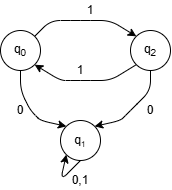
\includegraphics[width=0.3\textwidth]{Images/dfagraph.png}
                \end{center}
                Oppure dando una matrice di transizione
                \begin{center}
                    \begin{tabular}{|c|c|c|}
                        \hline
                         & 0 & 1 \\
                        \hline
                        $\displaystyle \to q_0$ & $q_1$ & $q_2$\\
                        \hline
                        $*q_1$& $q_1$ & $q_1$ \\
                        \hline
                        $q_2$ & $q_1$ & $q_0$ \\
                        \hline
                    \end{tabular}
                \end{center}
                Dove lo stato iniziale è indicato con $\to$ e lo stato finale con $*$.
                \begin{definitionbox}{Automa a stato finito non deterministico (NFA)}{}
                    E' una quintupla $\mathcal{M}=\langle Q,\Sigma, \delta, q_0, F\rangle$ dove $\delta:Q\times\Sigma\to\wp(Q)$.\\
                    $\wp(Q)$ mappa un \textbf{insieme di stati}, cioè l'insieme di tutti i sottoinsiemi possibili di $Q$. Ad esempio se abbiamo $Q=\{q_0,q_1,q_2\}$, $\wp(Q)=\left\{\{q_0\},\{q_1\},\{q_2\},\{q_0,q_1\},\ldots,\{q_0,q_1,q_2\}\right\}$
                \end{definitionbox}
                Analogamente ai DFA, un NFA può essere rappresentato in due modi principali:
                \begin{itemize}
                    \item \textbf{Grafo di transizione}: rimane concettualmente la stessa dei DFA
                    \item \textbf{Tabella di transizione}: ogni casella della tabella (corrispondente a una coppia stato/simbolo) può contenere un insieme di stati \begin{center}
                        \begin{tabular}{|c|c|c|}
                            \hline
                             & 0 & 1\\
                             \hline
                             $\to q_0$ & $\{q_0,q_1\}$ & $q_0$\\
                             \hline
                             $q_1$ & $\emptyset$ & $q_2$\\
                             \hline
                             $*q_2$ & $q_2$ & $q_2$\\
                            \hline
                        \end{tabular}
                    \end{center}
                \end{itemize}
                Il comportamento di un NFA è descritto da un sistema di transizione:
                \begin{itemize}
                    \item \textbf{Configurazioni}: Sono della forma $\langle q, u \rangle$, dove $q \in Q$ è lo stato corrente e $u \in \Sigma^*$ è la stringa ancora da leggere
                    \item \textbf{Relazione di riduzione}: È definita come: $\langle q, \sigma u \rangle \to \langle q', u \rangle$ se $q' \in \delta(q, \sigma)$. \textbf{Non è deterministica} ma comunque \textbf{terminante}, poichè a ogni passo viene consumato un simbolo di input (a meno che non si blocchi)
                    \item \textbf{Configurazioni di arresto}: Un NFA può bloccarsi in due modi: \begin{enumerate}
                        \item Quando ha letto tutta la stringa: $\langle q, \varepsilon \rangle$
                        \item Quando si trova in una configurazione $\langle q, \sigma u \rangle$ ma non esistono transizioni possibili per il simbolo $\sigma$ dallo stato $q$ (cioè $\delta(q, \sigma) = \emptyset$)
                    \end{enumerate}
                    \item \textbf{Direttive di Input/Output}: Le direttive di input/output sono simili a quelle dei DFA: \begin{itemize}
                        \item \textbf{Input}: $f_{IN}(u) = \langle q_0, u \rangle$
                        \item \textbf{Output}: $f_{OUT}=\begin{cases}
                            \langle q, u \rangle = \text{True} & \text{se }q \in F, u = \varepsilon\\
                            \text{False} & \text{altrimenti}
                        \end{cases}$
                    \end{itemize}
                    \item \textbf{Linguaggio Accettato}: Il linguaggio $L(\mathcal{M})$ accettato (o riconosciuto) da un NFA $\mathcal{M}$ è l'insieme delle stringhe $u$ per cui esiste almeno una computazione che, partendo dalla configurazione iniziale $\langle q_0, u \rangle$, raggiunge una configurazione $\langle q, \varepsilon \rangle$ dove $q$ è uno stato finale. Questo è un punto chiave del non determinismo: basta una computazione accettante tra tutte quelle possibili.\\
                    Un modo equivalente per definire il linguaggio accettato usa la funzione estesa $\hat{\delta} : Q \times \Sigma^* \to \wp(Q)$: \begin{itemize}
                        \item $\hat{\delta}(q, \varepsilon) = {q}$
                        \item $\hat{\delta}(q, u\sigma) = \bigcup_{q' \in \hat{\delta}(q, u)} \delta(q', \sigma)$
                    \end{itemize}
                    Con questa definizione, una stringa $u$ è accettata se e solo se esiste uno stato $q$ nell'insieme $\hat{\delta}(q_0, u)$ che sia uno stato finale ($q \in F$). In altre parole, $L(\mathcal{M}) = {u \mid \hat{\delta}(q_0, u) \cap F \neq \emptyset }$
                \end{itemize}
                \begin{theorembox}{Rabin-Scott}{}
                    Sia $\mathcal{M}=\langle Q,\Sigma,\delta_N,q_0,F_N\rangle$ un NFA. Allora esiste un DFA $\mathcal{M}_D$ tale che $L(\mathcal{M}_D)=L(\mathcal{M})$
                \end{theorembox}
                \textbf{Prova}: Costruiamo $\mathcal{M}_D$ come la quintupla $\langle\wp(Q),\Sigma,\delta_D,\{q_0\},F_D\rangle$. L'idea centrale della costruzione è che ogni stato del nuovo DFA $\mathcal{M}_D$ corrisponde a un insieme di stati dell'NFA originale.
                \begin{itemize}
                    \item $Q_D=\wp(Q_N)$: questo significa che ogni stato del DFA è un sottoinsieme degli stati dell'NFA. Se l'NFA ha $|Q_N|$ stati, il DFA risultante può avere fino a $2^{|Q_N|}$ stati, sebbene non tutti siano necessariamente raggiungibili.
                    \item $\delta_D$: per ogni stato $q_D\in\wp(Q_N)$ (che è un insieme di stati dell'NFA) e per ogni simbolo $\sigma \in \Sigma$, la transizione $\delta_D(q_D, \sigma)$ porta a un nuovo stato del DFA che è l'unione di tutti gli stati raggiungibili nell'NFA da qualsiasi stato in $q_D$ leggendo $\sigma$. Formalmente: \begin{equation*}
                        \delta_D(q_D, \sigma) = \bigcup_{q \in q_D} \delta_N(q, \sigma)
                    \end{equation*}
                    \item $F_D$: Uno stato $q_D \subseteq Q_N$ del DFA è uno stato finale se e solo se contiene almeno uno stato finale dell'NFA. Formalmente: \begin{equation*}
                        F_D = {q_D \subseteq Q_N \mid q_D \cap F_N \neq \emptyset}
                    \end{equation*}
                \end{itemize}
                \begin{example}{}
                    \begin{itemize}
                        \item \textbf{NFA Originale $\left(\mathcal{M}_N\right)$}: $\mathcal{M}=\left(\{q_0,q_1,q_2\},\{0,1\},\delta_N,q_0,q_2\right)$ con \begin{center}
                            $\delta_N=$ \begin{tabular}{|c|c|c|}
                                \hline
                                & 0 & 1 \\
                                \hline
                                $\to q_0$ & $q_0$ & $\{q_0,q_1\}$\\
                                \hline
                                $q_1$ & $\emptyset$ & $q_2$\\
                                \hline
                                $*q_2$ & $q_2$ & $q_2$\\
                                \hline
                            \end{tabular}
                        \end{center}
                        \item \textbf{DFA Derivante $(\mathcal{M}_D)$}: $\mathcal{M}_D=(Q_D,\{0,1\},\delta_D,q_0,F_D)$ \begin{itemize}
                            \item $Q_D=\{\emptyset,\{q_0\},\{q_1\},\{q_2\},\{q_0,q_1\},\{q_0,q_2\},\{q_1,q_2\},\{q_0,q_1,q_2\}\}$
                            \item $F_D=\{\{q_2\},\{q_0,q_2\},\{q_1,q_2\},\{q_0,q_1,q_2\}\}$ (tutti gli stati che contengono lo stato finale della NFA)
                            \item $\delta_D$: \begin{enumerate}
                                \item \textbf{Da $\{q_0\}$}: \begin{itemize}
                                    \item $\delta_D(q_0,0)=\delta_N(q_0,0)=q_0$
                                    \item $\delta_D(q_0,1)=\delta_N(q_0,1)=\{q_0,q_1\}$
                                \end{itemize}
                                \item \textbf{Da $\{q_0,q_1\}$}: \begin{itemize}
                                    \item $\delta_D(\{q_0,q_1\},0)=\delta_N(q_0,0)\cup \delta_N(q_1,0)=\{q_0\}\cup\emptyset=q_0$
                                    \item $\delta_D(\{q_0,q_1\},1)=\delta_N(q_0,1)\cup \delta_N(q_1,1)=\{q_0,q_1\}\cup\{q_2\}=\{q_0,q_1,q_2\}$ 
                                \end{itemize}
                                \item \textbf{Da $\{q_0,q_1,q_2\}$}: \begin{itemize}
                                    \item $\delta_D(\{q_0,q_1,q_2\},0)=\delta_N(q_0,0)\cup \delta_N(q_1,0)\cup\delta_N(q_2,0)=\{q_0\}\cup\emptyset\cup\{q_2\}=\{q_0,q_2\}$
                                    \item $\delta_D(\{q_0,q_1,q_2\},1)=\delta_N(q_0,1)\cup \delta_N(q_1,1)\cup\delta_N(q_2,1)=\{q_0,q_1\}\cup\{q_2\}\cup\{q_2\}=\{q_0,q_1,q_2\}$
                                \end{itemize}
                                \item \textbf{Da $\{q_0,q_2\}$}: \begin{itemize}
                                    \item $\delta_D(\{q_0,q_2\},0)=\delta_N(q_0,0)\cup \delta_N(q_2,0)=\{q_0\}\cup\{q_2\}=\{q_0,q_2\}$
                                    \item $\delta_D(\{q_0,q_2\},1)=\delta_N(q_0,1)\cup \delta_N(q_2,1)=\{q_0,q_1\}\cup\{q_2\}=\{q_0,q_1,q_2\}$
                                \end{itemize}
                            \end{enumerate}
                            Quindi \begin{center}
                                $\delta_D=$ \begin{tabular}{|c|c|c|}
                                \hline
                                & 0 & 1 \\
                                \hline
                                $\to q_0$ & $q_0$ & $\{q_0,q_1\}$\\
                                \hline
                                $\{q_0,q_1\}$ & $q_0$ & $\{q_0,q_1,q_2\}$\\
                                \hline
                                $*\{q_0,q_1,q_2\}$ & $\{q_0,q_2\}$ & $\{q_0,q_1,q_2\}$\\
                                \hline
                                $*\{q_0,q_2\}$ & $\{q_0,q_2\}$ & $\{q_0,q_1,q_2\}$\\
                                \hline
                            \end{tabular}
                            \end{center}
                        \end{itemize}
                    \end{itemize}
                    \textit{Abbiamo costruito la tabella includendo unicamente gli stati raggiungibili a partire da $\{q_0\}$. Secondo la definizione di $\delta_D$, non è necessario calcolare le transizioni per stati come $\{q_1\}$, $\{q_1,q_2\}$ e $\{q_2\}$, dato che non vengono mai raggiunti.}
                \end{example}
                \begin{demonstration}
                    \large\textbf{Dimostrazione per induzione}\normalsize\\
                    \textbf{Base}
                    \begin{itemize}
                        \item Per la definizione della funzione di transizione estesa in un DFA, $\hat{\delta}_D({q_0}, \varepsilon) = {q_0}$
                        \item Per la definizione della funzione di transizione estesa in un NFA, $\hat{\delta}_N(q_0, \varepsilon) = {q_0}$
                    \end{itemize}
                    Quindi, la condizione è soddisfatta per la stringa vuota: $\hat{\delta}_D({q_0}, \varepsilon) = \hat{\delta}_N(q_0, \varepsilon)$.\\
                    \textbf{Passo (Stringa $u\sigma$)}
                    \begin{itemize}
                        \item Assumiamo, per ipotesi induttiva, che per una generica stringa $u$, valga $\hat{\delta}_D({q_0}, u) = \hat{\delta}_N(q_0, u)$, vogliamo dimostrare che la stessa uguaglianza vale per la stringa $u\sigma$
                        \item Applichiamo la definizione di $\hat{\delta}_D$ a $u\sigma$: $\hat{\delta}_D({q_0}, u\sigma) = \delta_D(\hat{\delta}_D({q_0}, u), \sigma)$, possiamo sostituire $\hat{\delta}_D({q_0}, u)$ con $\hat{\delta}_N(q_0, u)$: $= \delta_D(\hat{\delta}_N(q_0, u), \sigma)$
                        \item Ora applichiamo la definizione di $\delta_D$: è l'unione delle transizioni $\delta_N(q', \sigma)$ per tutti gli stati $q'$ nell'insieme $\hat{\delta}_N(q_0, u)$:$= \bigcup_{q' \in \hat{\delta}_N(q_0, u)} \delta_N(q', \sigma)$. Questa è precisamente la definizione di $\hat{\delta}_N(q_0, u\sigma)$
                    \end{itemize}
                    Quindi, $\hat{\delta}_D({q_0}, u\sigma) = \hat{\delta}_N(q_0, u\sigma)$.\\
                    Avendo dimostrato per induzione che $\hat{\delta}_D({q_0}, u) = \hat{\delta}_N(q_0, u)$ per ogni stringa $u \in \Sigma^*$, possiamo concludere sull'accettazione del linguaggio:
                    \begin{itemize}
                        \item Una stringa $u$ è accettata dal DFA $\mathcal{M}_D$ se e solo se $\hat{\delta}_D({q_0}, u) \in F_D$
                        \item Per definizione di $F_D$, ciò significa che $\hat{\delta}_D({q_0}, u)$ deve contenere almeno uno stato finale di $\mathcal{M}_N$, ovvero $\hat{\delta}_D({q_0}, u) \cap F_N \neq \emptyset$
                        \item Poiché $\hat{\delta}_D({q_0}, u) = \hat{\delta}_N(q_0, u)$, questo è equivalente a $\hat{\delta}_N(q_0, u) \cap F_N \neq \emptyset$
                        \item E quest'ultima è la condizione di accettazione di una stringa per un NFA $\mathcal{M}_N$
                    \end{itemize}
                    Pertanto, $u$ è accettata da $\mathcal{M}_D$ se e solo se è accettata da $\mathcal{M}_N$, il che significa che $L(\mathcal{M}_D) = L(\mathcal{M}_N)$.
                \end{demonstration}
                \begin{definitionbox}{$\varepsilon$-NFA o NFA con transizioni silenti}{}
                    E' una quintupla $M = \langle Q, \Sigma, \delta, q_0, F \rangle$ dove la funzione di transizione, che ha la forma \begin{equation*}
                        \delta : Q \times (\Sigma \cup \{\varepsilon\}) \to \wp(Q)
                    \end{equation*}
                    La peculiarità di questa definizione è l'inclusione di $\varepsilon$ nell'alfabeto di input della funzione di transizione, il che consente transizioni tra stati senza consumare alcun simbolo di input (transizioni silenti). Questo permette, in molti casi, di costruire automi più semplici e leggibili
                \end{definitionbox}
                Il comportamento di un $\varepsilon$-NFA è descritto da un sistema di transizione con le seguenti caratteristiche:
                \begin{itemize}
                    \item \textbf{Configurazioni}: Sono della forma $\langle q, u \rangle$, dove $q \in Q$ è lo stato corrente e $u \in \Sigma^*$ è la stringa ancora da leggere
                    \item \textbf{Relazione di riduzione}: È definita in due modi: \begin{itemize}
                        \item $\langle q, \sigma u \rangle \to \langle q', u \rangle$ se $q' \in \delta(q, \sigma)$ (transizione standard, consumando un simbolo)
                        \item $\langle q, u \rangle \to \langle q', u \rangle$ se $q' \in \delta(q, \varepsilon)$ (transizione silente, senza consumare simboli)
                    \end{itemize}
                    La relazione di riduzione è non deterministica, anche per via della possibilità di scegliere tra leggere o non leggere un simbolo. È generalmente non terminante, ma le computazioni infinite sono dovute solo a cicli di transizioni $\varepsilon$ dallo stesso stato, che possono essere eliminati.
                    \item \textbf{Configurazione di arresto}: Oltre alle configurazioni della forma $\langle q, \varepsilon \rangle$, includono anche quelle in cui l'automa si blocca perché non ci sono transizioni possibili (né con simboli di input, né silenti) da un dato stato con il simbolo corrente
                    \item \textbf{Linguaggio accettato}: Le direttive di input/output sono le stesse degli NFA. Una stringa $u$ è accettata se esiste almeno una computazione che, partendo dalla configurazione iniziale $\langle q_0, u \rangle$, raggiunge una configurazione $\langle q, \varepsilon \rangle$ dove $q$ è uno stato finale. Un modo equivalente per definire il linguaggio accettato utilizza la funzione di transizione estesa $\hat{\delta} : Q \times \Sigma^* \to \wp(Q)$, che si basa sul concetto di $\varepsilon$-closure: \begin{itemize}
                        \item \textbf{$\varepsilon-closure(q)$}: È l'insieme di tutti gli stati raggiungibili da $q$ utilizzando zero o più transizioni $\varepsilon$. Formalmente, include $q$ stesso, tutti gli stati raggiungibili da $q$ tramite $\delta(q, \varepsilon)$, e ricorsivamente tutti gli stati raggiungibili da questi ultimi tramite ulteriori transizioni $\varepsilon$
                        \item \textbf{Funzione di transizione estesa $\hat{\delta}$}: \begin{itemize}
                            \item $\hat{\delta}(q, \varepsilon) = \varepsilon\text{-closure}(q)$
                            \item $\hat{\delta}(q, u\sigma) = \bigcup_{q' \in \hat{\delta}(q, u)} \varepsilon\text{-closure}(\delta(q', \sigma))$
                        \end{itemize}
                        Una stringa $u$ è accettata se e solo se l'insieme di stati raggiungibili dopo aver letto $u$ (cioè $\hat{\delta}(q_0, u)$) contiene almeno uno stato finale ($\hat{\delta}(q_0, u) \cap F \neq \emptyset$)
                    \end{itemize}
                \end{itemize}
                \begin{example}
                    $\mathcal{M}_N=(\{q_0,q_1,q_2\},\{a,b\},\delta_N,q_0,F_N)$
                    \begin{center}
                        $\delta_N=$ \begin{tabular}{|c|c|c|c|}
                            \hline
                             & a & b & $\varepsilon$\\
                            \hline
                            $\to q_0$ & \ldots & \ldots & $q_1$\\
                            \hline
                            $q_1$ & \ldots & \ldots & $q_2$\\
                            \hline
                            $*q_2$ & \ldots & \ldots & $q_1$\\
                            \hline
                        \end{tabular}
                    \end{center}
                    \textbf{Calcolo le $\varepsilon-closure$}: \begin{itemize}
                        \item $\varepsilon-closure(q_0)=\{q_0,q_1,q_2\}$
                        \item $\varepsilon-closure(q_1)=\{q_1,q_2\}$
                        \item $\varepsilon-closure(q_2)=\{q_2,q_1\}$
                    \end{itemize}
                \end{example}

\end{document}